\begin{fact}\label{iso-tri}
	Considérons tous les triangles de périmètre fixé $p$. Parmi tous ces triangles, celui d'aire maximale est le triangle équilatéral de côté $c = \dfrac13 p$.
\end{fact}


\begin{proof}
	Une première idée, calculatoire, est de passer via la classique formule de Héron $Aire = \sqrt{s(s - a)(s - b)(s - c)}$ où $s = \num{.5} p$ désigne le demi-périmètre, et les variables $a$, $b$ et $c$ les mesures des côtés du triangle,%
	\footnote{
		L'aire étant positive ou nulle, nous devons chercher les maxima de $f(a;b;c) = Aire^2 = s(s - a)(s - b)(s - c)$, c'est-à-dire de $f(a;b;c) = \frac{1}{16} (a + b + c)(b + c - a)(a + c - b)(a + b - c)$, sous la contrainte $2s = a + b + c$ où $s > 0$ est constant.
		Notant $g(a;b;c) = a + b + c - 2 s$, la contrainte s'écrit $g(a;b;c) = 0$.
		Selon la méthode des extrema liés, un éventuel maximum doit vérifier 
		$\pder[i]{f}{a}{1} = \lambda \pder[i]{g}{a}{1}$,
		$\pder[i]{f}{b}{1} = \lambda \pder[i]{g}{b}{1}$ et
		$\pder[i]{f}{c}{1} = \lambda \pder[i]{g}{c}{1}$
		avec $\lambda \in \RR$.
		Donc,
		$- s(s - b)(s - c) = - s(s - a)(s - c) = - s(s - a)(s - b) = \lambda$,
		puis
		$(s - b)(s - c) = (s - a)(s - c) = (s - a)(s - b)$.
		Les cas $s = a$, $s = b$ et $s = c$ donnent $f(a;b;c) = 0$.
		Quant au cas $\big[ s \neq a, s \neq b \text{ et } s \neq c \big]$, il n'est envisageable que si $a = b = c = \frac{p}{3}$ qui implique $f(a;b;c) = \frac{1}{16} p \big( \frac{p}{3} \big)^3 = \big( \frac{p^2}{12 \sqrt{3}} \big)^2 > 0$.
		En résumé, l'existence d'un maximum implique que ce maximum corresponde au cas du triangle équilatéral.
		Il reste à démontrer qu'un tel maximum existe pour pouvoir conclure: ceci est facile à justifier en considérant l'ensemble compact $\intervalC{0}{s}^3$ de $\RR^3$. 
	}
	mais il se trouve que l'on peut raisonner plus géométriquement comme suit.
	%
	Partant d'un triangle $ABC$ quelconque de périmètre $p$, le fait \ref{iso-tri} nous donne successivement les triangles $ACD$, $ADE$ et $AEF$ isocèles en $D$, $E$ et $F$ respectivement, ayant tous pour périmètre $p$, et ceci avec des aires de plus en plus grandes.  
	Le dessin suivant amène à conjecturer qu'en poursuivant le procédé pour avoir ensuite un triangle $AFG$ isocèle en $G$...\,, nous aboutirons \og \emph{à la limite} \fg\ à un triangle équilatéral.

	\begin{center}
		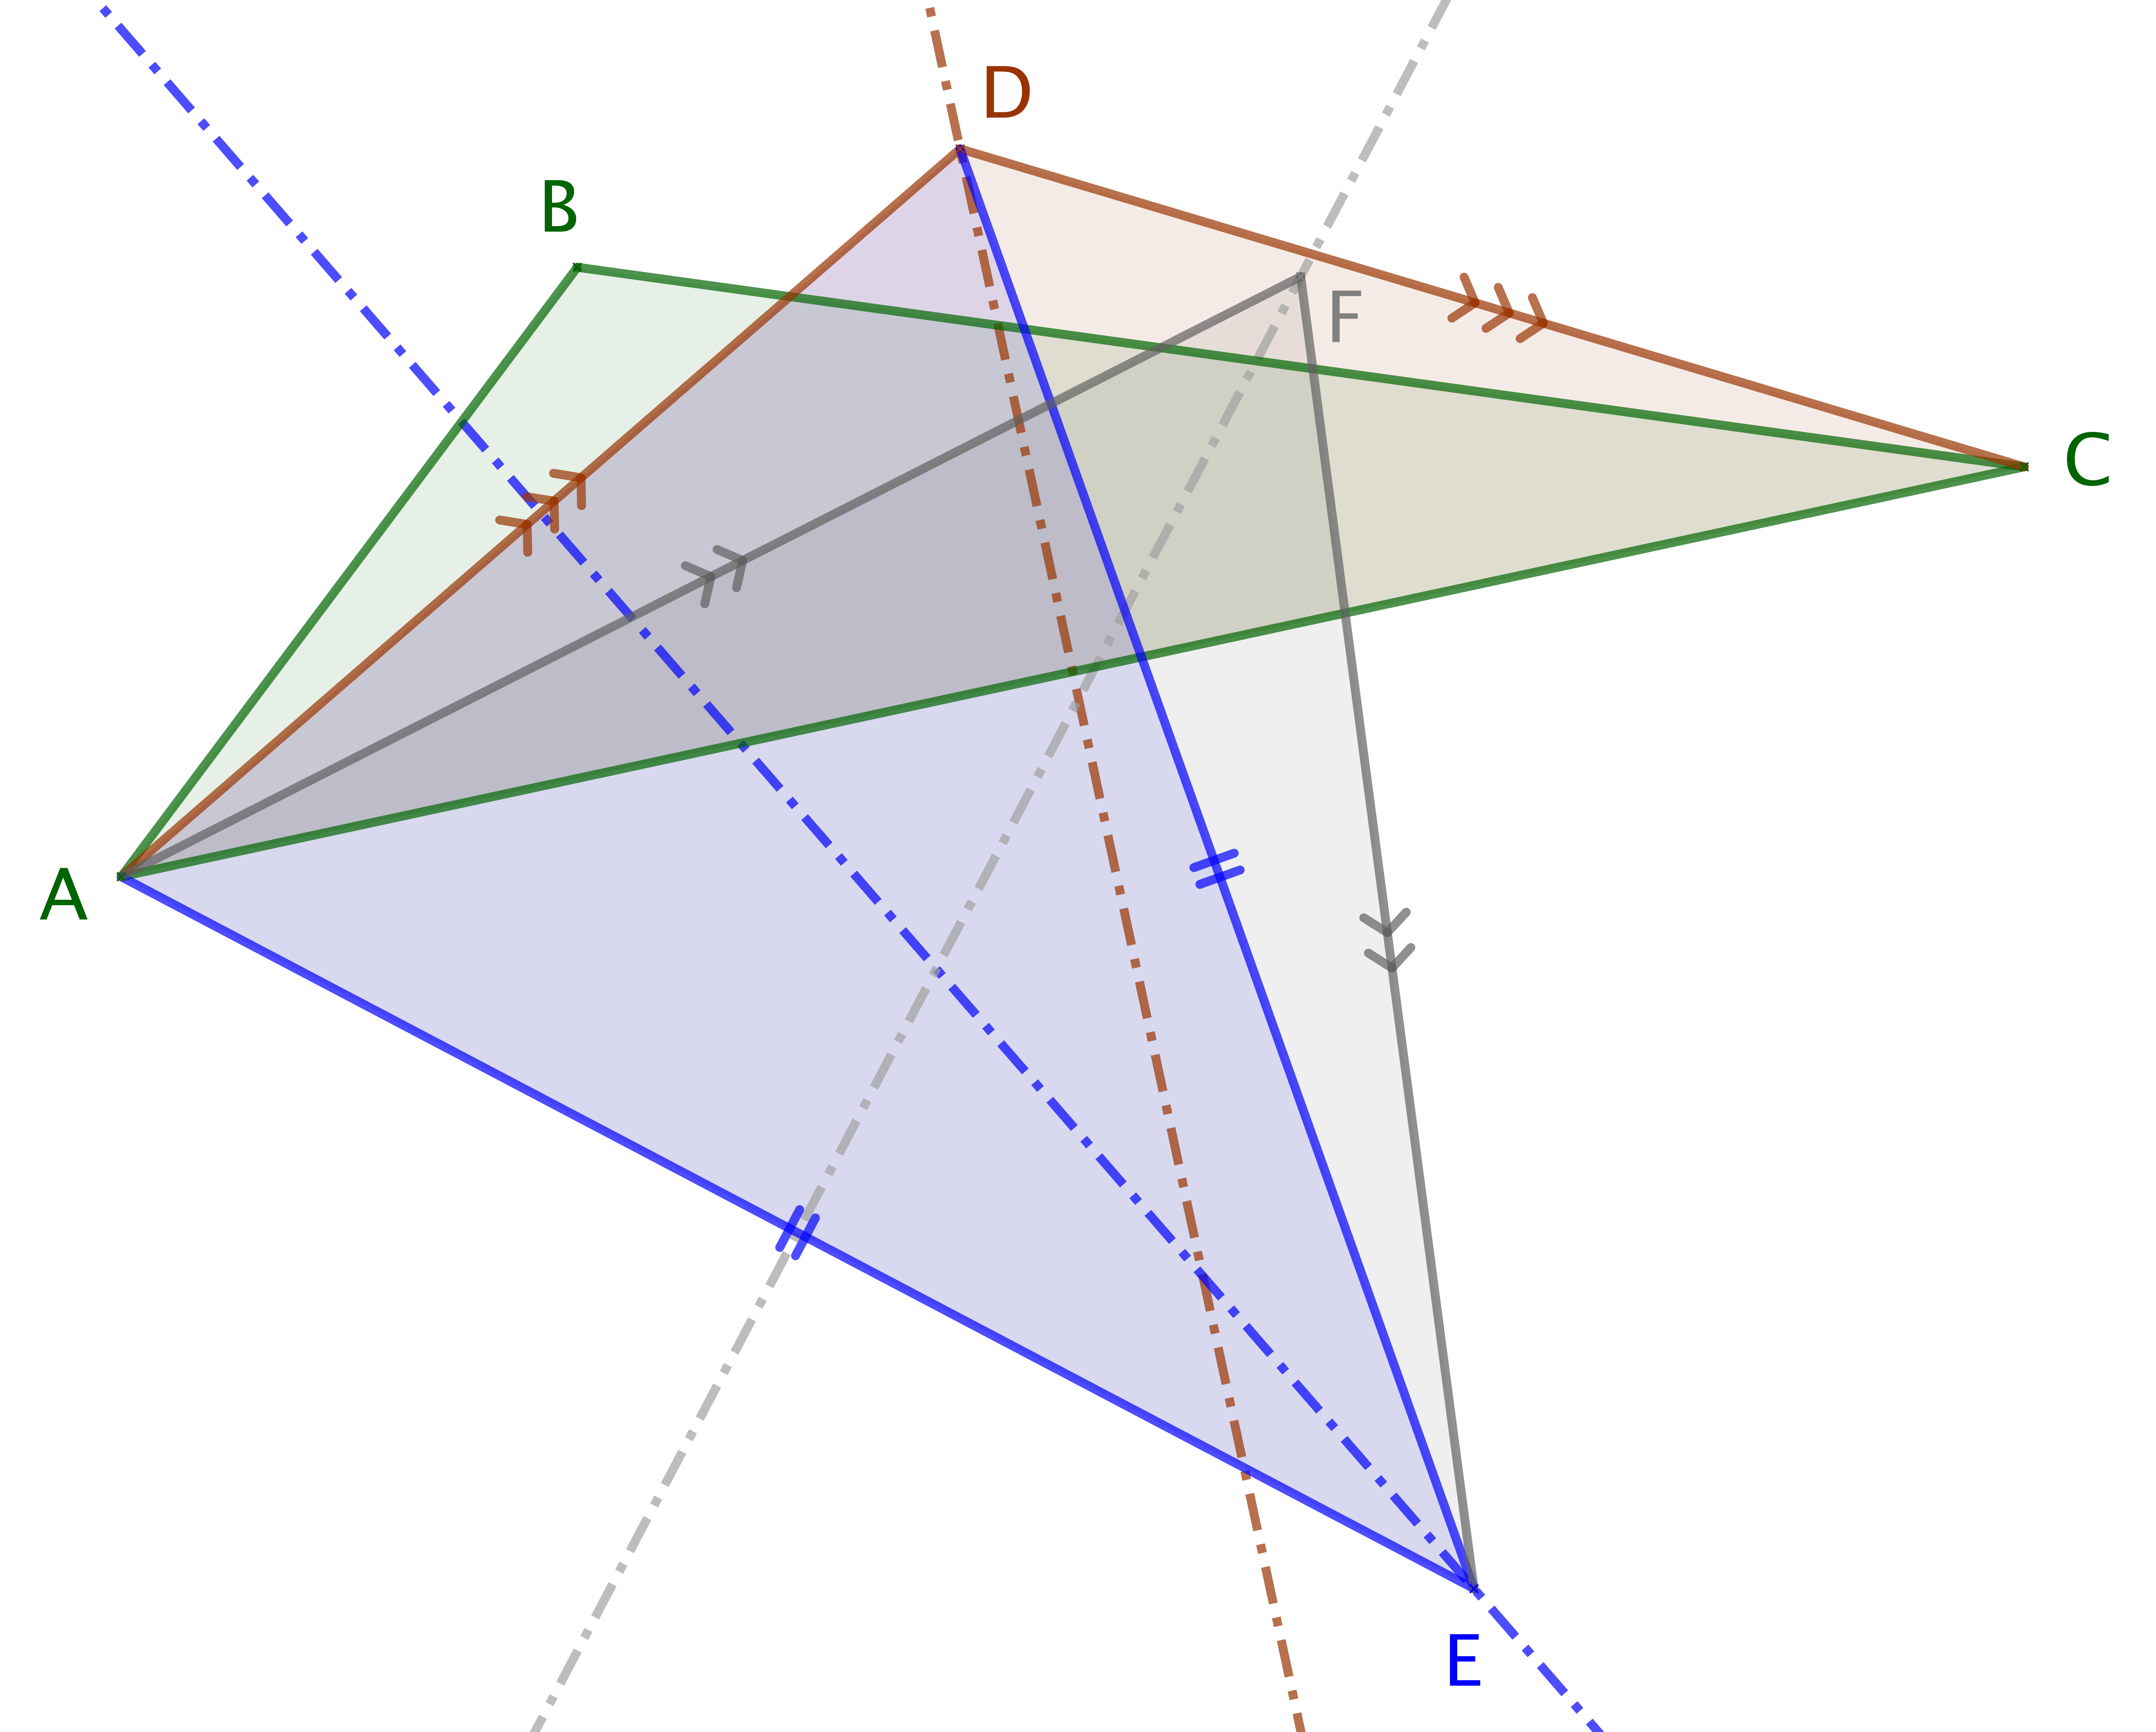
\includegraphics[scale=.4]{content/triangle-gene/triangle-conj.png}
	\end{center} 

	
	Le passage d'un triangle quelconque $ABC$ au triangle $ACD$ isocèle en $D$ nous amène à nous concentrer sur ce que donne notre procédé d'agrandissement d'aire à périmètre fixé lorsque l'on passe de $ADC$ à $ADE$ en partant d'un triangle isocèle. Représentons juste cette étape, avec $ADC$ non équilatéral, pour y voir plus clair.

	\begin{center}
		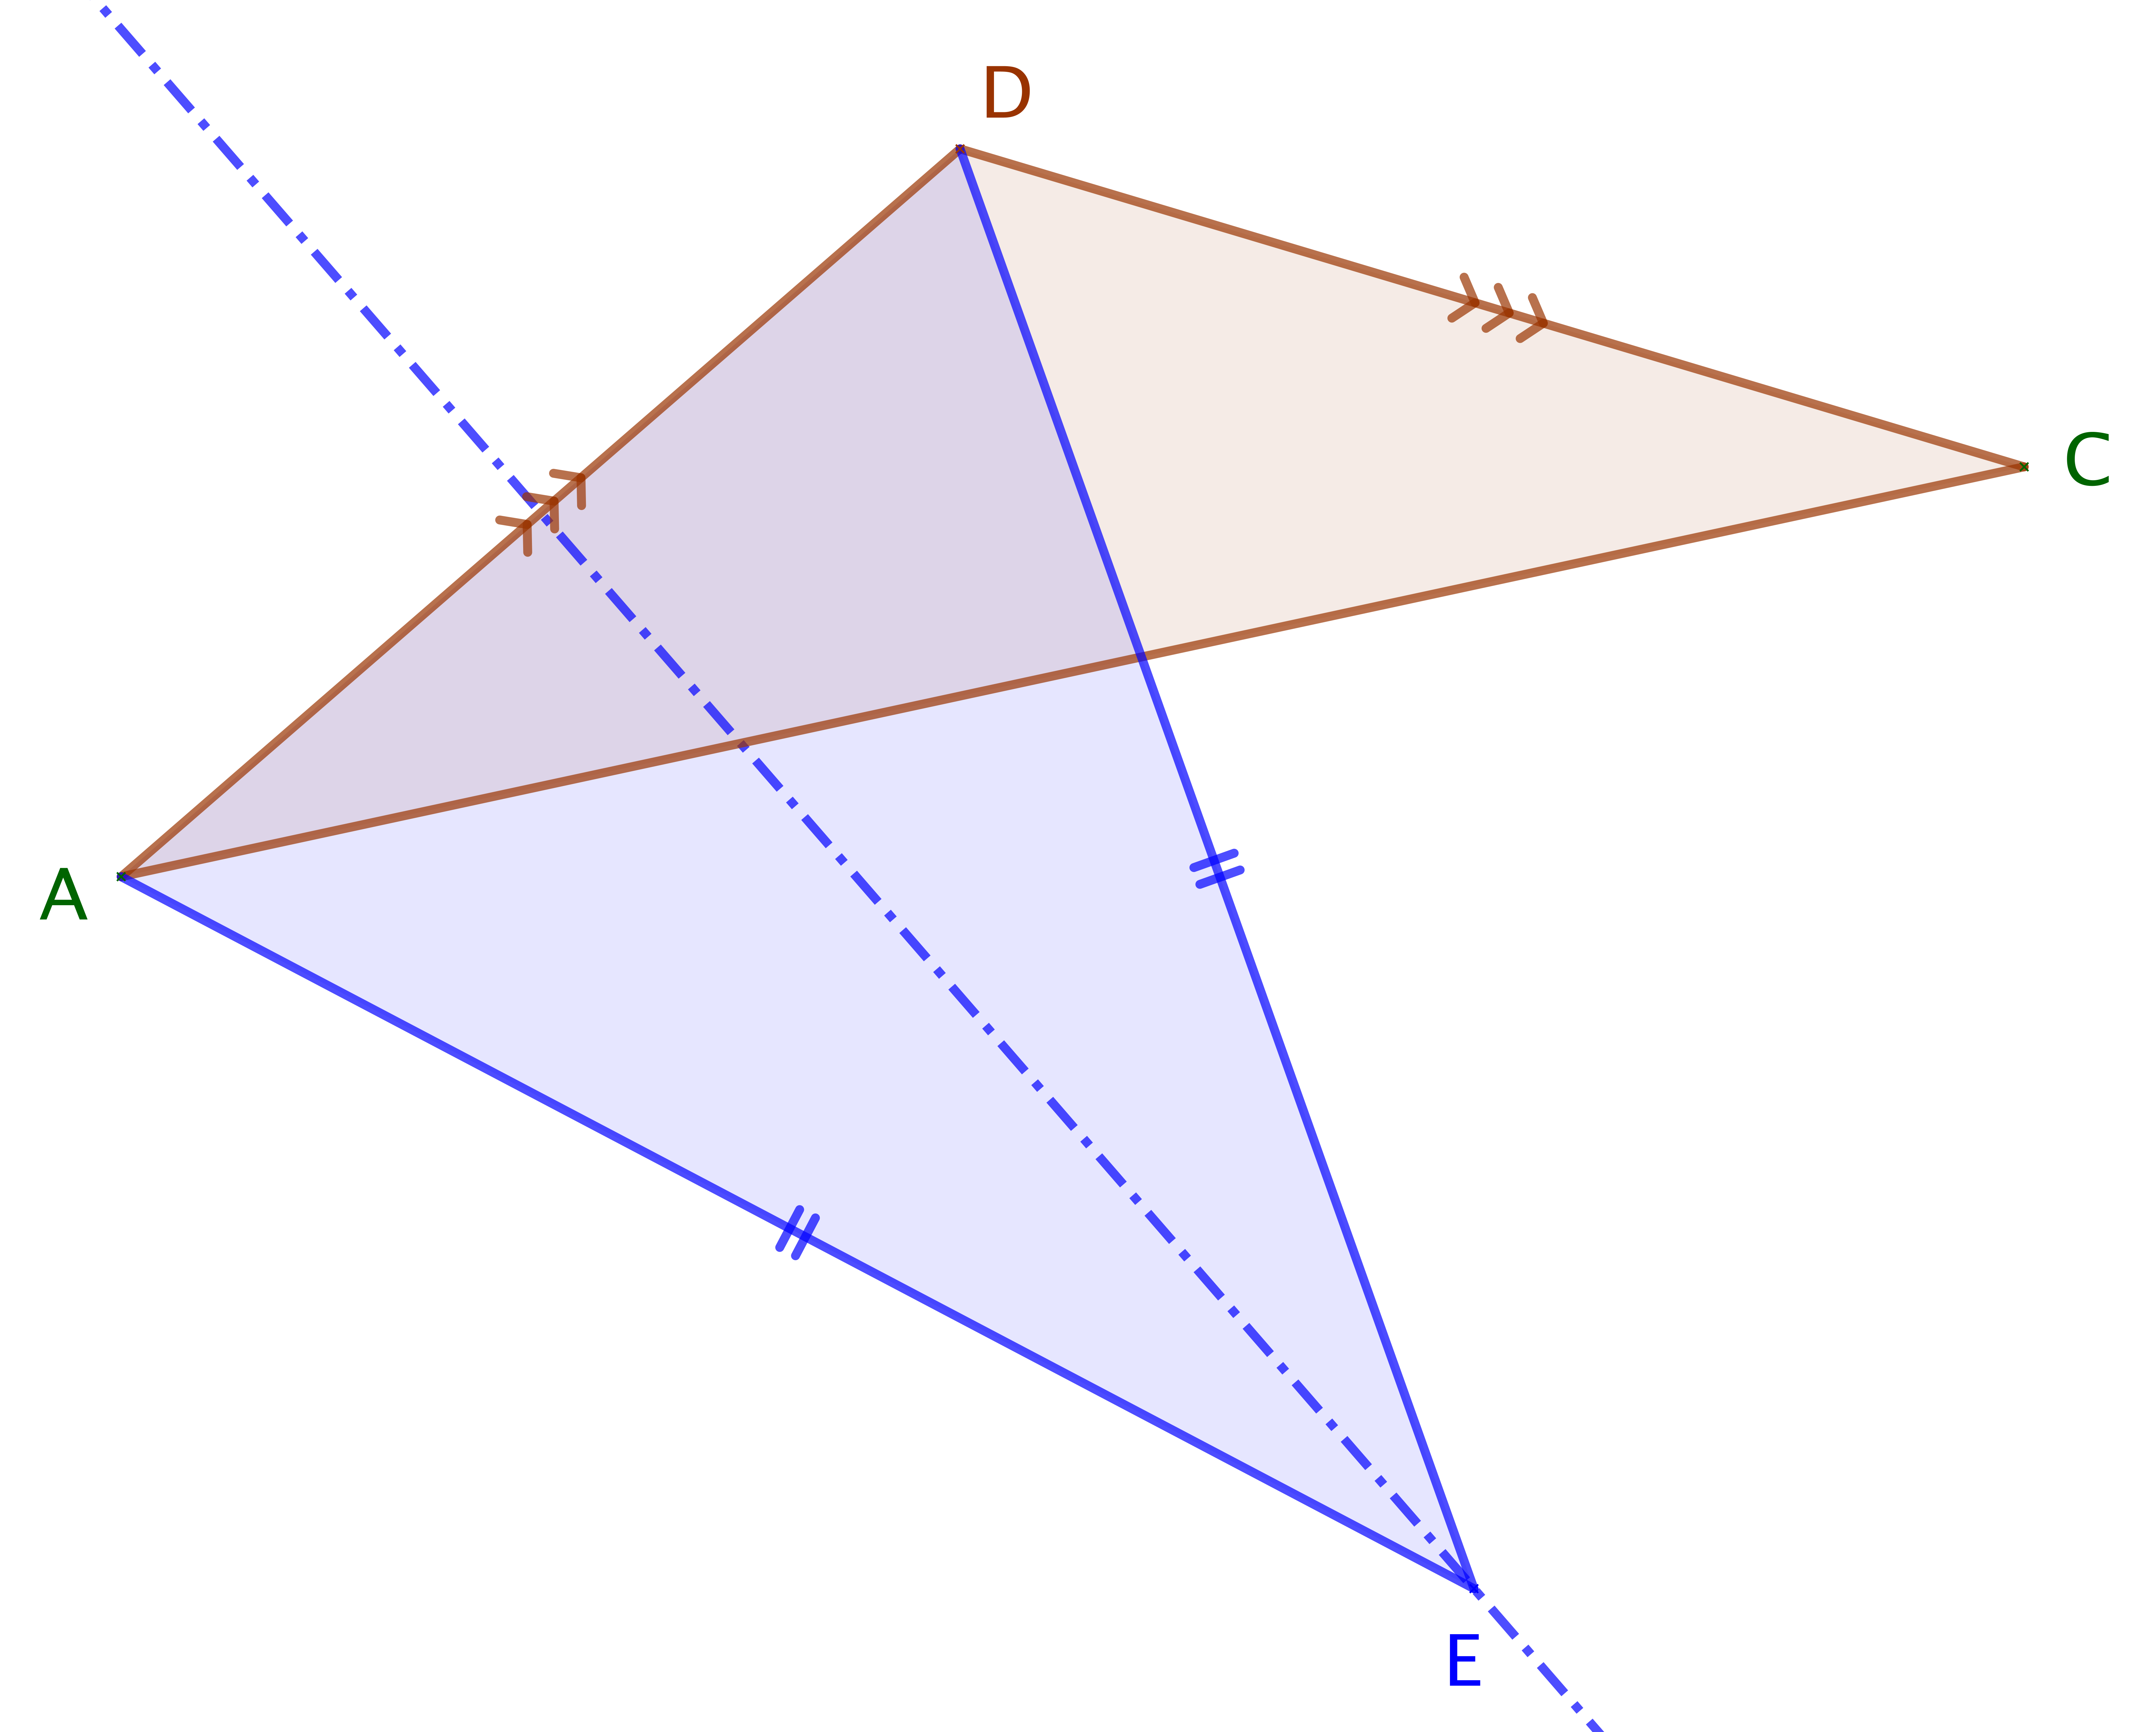
\includegraphics[scale=.4]{content/triangle-gene/triangle-proof.png}
	\end{center} 
	
	
	Notons que si $ADC$ est équilatéral, notre construction s'arrête.
	Nous supposons donc le contraire dans la suite.


		\item Notre construction nous donne forcément si $ADC$ n'est pas équilatéral.


\end{proof}


% ----------------------- %


\begin{remark}
	La comparaison des moyennes géométriques et arithmétiques d'ordre $3$ nous donne une solution algébrique efficace, car 
	$\sqrt[3]{(s - a)(s - b)(s - c)} \leq \frac13 \big( (s - a) + (s - b) + (s - c) \big)$
	nous donne
	$s(s - a)(s - b)(s - c) \leq \frac{1}{27} s^4$,
	puis
	$\sqrt{s(s - a)(s - b)(s - c)} \leq \frac{p^2}{12 \sqrt{3}}$
	où $\frac{p^2}{12 \sqrt{3}}$ est l'aire du triangle équilatéral de périmètre $p$.
\end{remark}
